The function \texttt{getaddrinfo(\ldots)} resolves a service name to a list of
endpoints in an order that prioritizes an IPv6-upgrade path \cite{rfc6724}.
The order can dramatically reduce the application's responsiveness where IPv6
connectivity is broken, because the attempt to connect over an IPv4 endpoint
will take place only when the IPv6 connection attempt has timed out, which can
be in the order of seconds.

\begin{figure}[t]
\centering
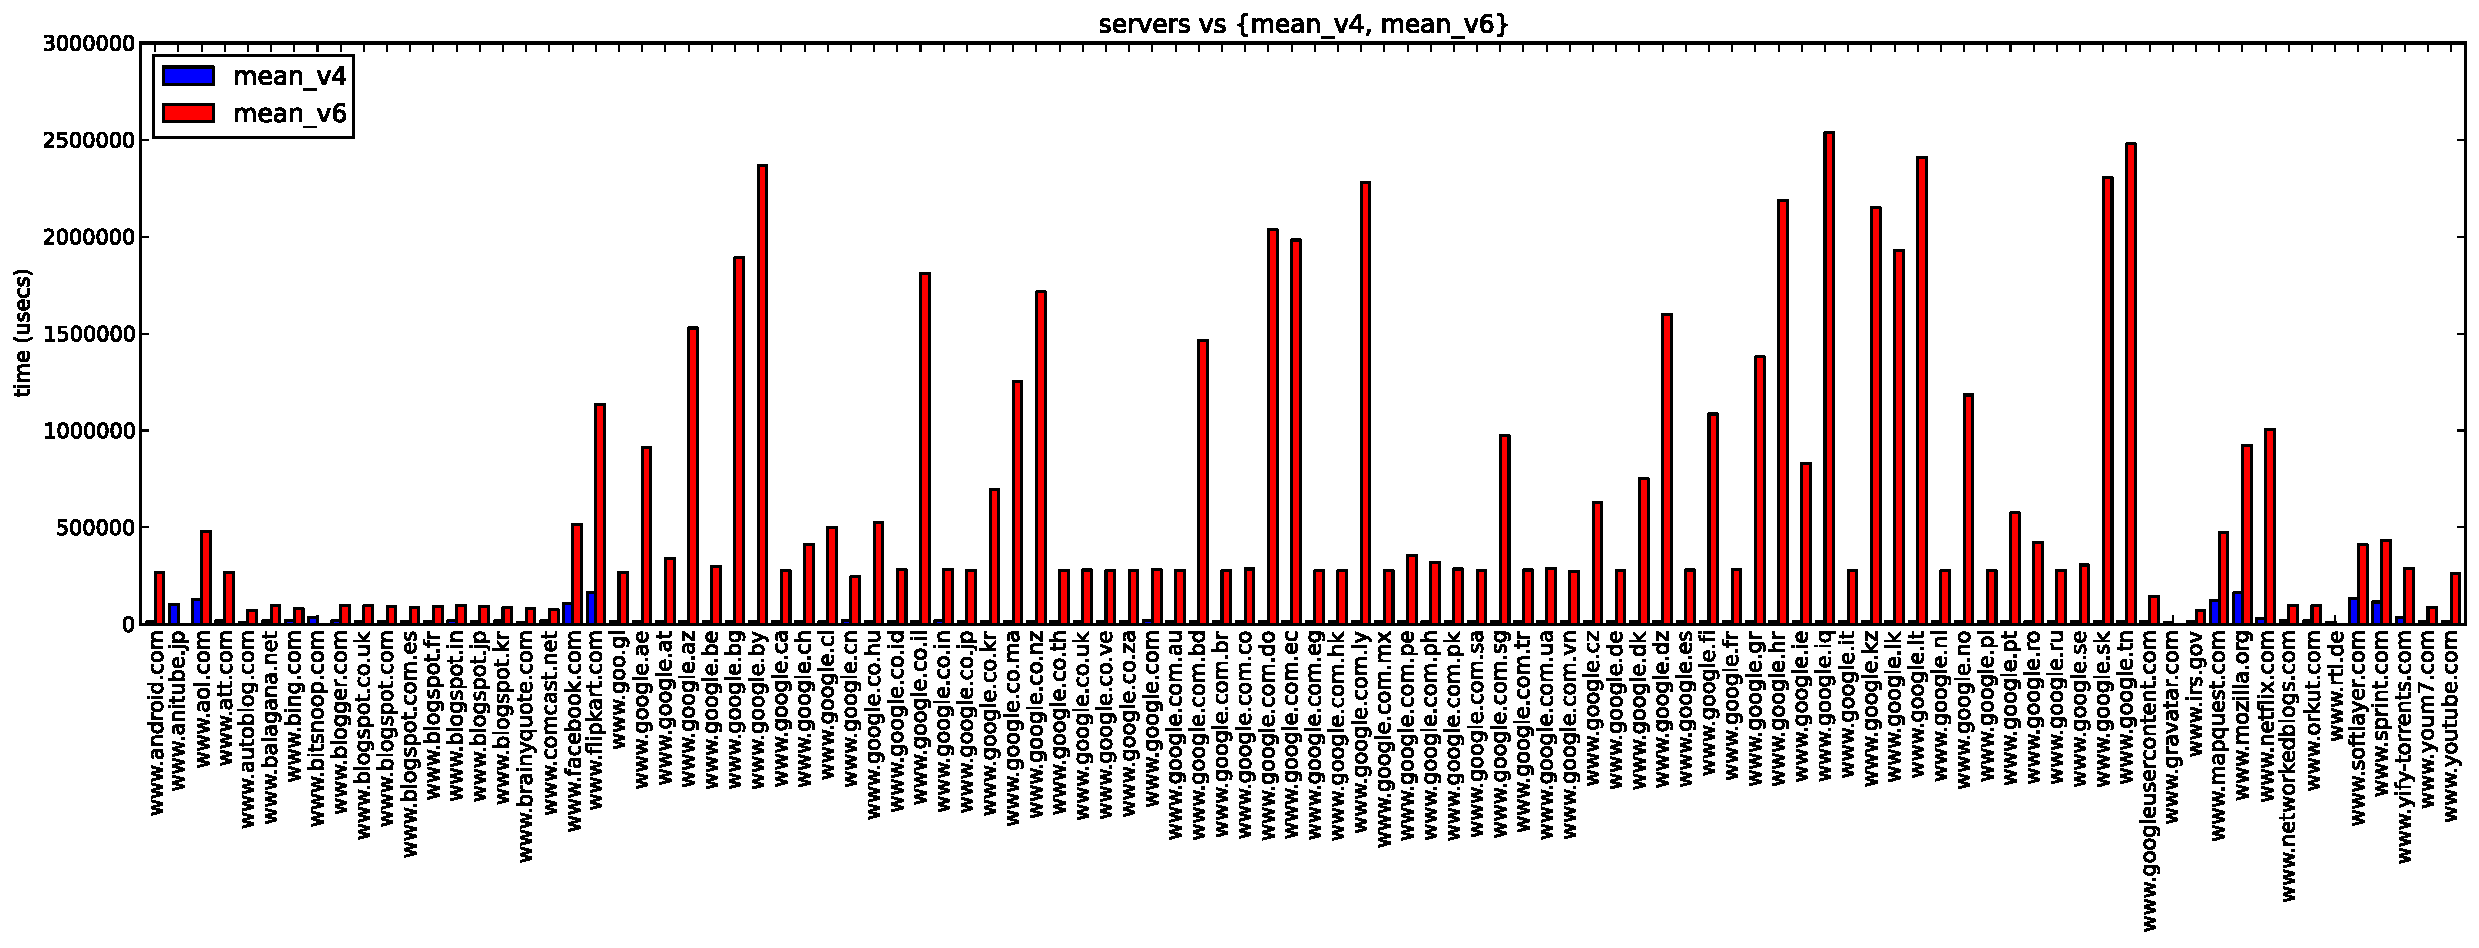
\includegraphics[width=1.0\textwidth]{figures/t28972-mean}
\caption{Mean time to establish TCP connections to a list of web services. The
\ac{MA} is a virtual machine hosted at \texttt{greatnet.de}. It has IPv4
connectivity via LamdaNet Communications [AS13237] and IPv6 connectivity via
Teredo.}
\label{fig:t28972-mean}
\end{figure}

This degraded user experience can be subverted by implementing the happy
eyeballs algorithm \cite{rfc6555}. The algorithm recommends that a host, after
resolving the service name, tries a TCP \texttt{connect(\ldots)} to the first
endpoint (usually IPv6). However, instead of waiting for a timeout, it only
waits for 300ms, after which it must initiate another TCP
\texttt{connect(\ldots)} to an endpoint with a different address family and
start a competition to pick the one that completes first. We have developed
\texttt{happy}, a simple TCP happy eyeballs probing tool that uses TCP
connection establishment time as a parameter to measure the algorithm's
effectiveness. It uses non-blocking \texttt{connect(\ldots)} calls to
concurrently establish connections to all endpoints of a service. In order to
develop data-analysis tools, we have prepared an internal test-bed of multiple
\ac{MA}s. The \ac{MA}s have different flavors of IPv4 and IPv6 connectivity
ranging from native IPv4, native IPv6, IPv6 tunnel broker endpoints, Teredo
and tunnelled IPv4. We used the top 100 DNS names compiled by
\texttt{he.net}\footnote{\url{http://bgp.he.net/ipv6-progress-report.cgi}} and
ran \texttt{happy} on them.

A preliminary result comparing the mean time to establish a TCP connection to
each of the services from one of the \ac{MA} is shown in Fig.
\ref{fig:t28972-mean}. The initial results show higher connection times over
IPv6. Furthermore, on a Teredo \ac{MA}, an application will never use IPv6
except when IPv4 connectivity is broken, because the Teredo IPv6 prefix has a
low priority in the address selection algorithm \cite{rfc6724}. It also
appears that several services show very similar performance. These services
resolve to a set of endpoints that belong to the same allocated address
blocks. Digging through the \texttt{whois} information for each of the
endpoints from their \ac{RIR} demonstrates that major portions of the services
map to address blocks owned by organizations such as Google and Akamai
Technologies.
